\documentclass[12pt,a4paper]{article}

\usepackage[english]{babel}
\usepackage[utf8x]{inputenc}
\usepackage{amsmath}
\usepackage{setspace}
\usepackage{graphicx}
\usepackage{float}
\usepackage{amssymb}
\usepackage{geometry}
\usepackage{indentfirst}
\usepackage{mathpazo}
\usepackage{varwidth}
\usepackage{algorithm}  
\usepackage{algorithmic}
\usepackage{tikz}
\usepackage{subcaption}

\geometry{left=2.54cm,right=2.54cm,top=2.54cm,bottom=2.54cm}

\title{EECS 442 F14\\HW \# 5}
\author{WU Tongshuang 40782356}
\date{\today}
\setlength{\parskip}{0.5\baselineskip}

\begin{document}
%\maketitle

\tikzstyle{hidden} = [circle, thin, draw=red, minimum size=10mm,inner sep=0pt]
\tikzstyle{start} = [circle, thin, draw=blue, minimum size=10mm,inner sep=0pt]
\tikzstyle{dev} = [circle, thin, draw=white, minimum size=10mm,inner sep=0pt]

\tikzstyle{final} = [circle, thin, draw=blue, minimum size=10mm,inner sep=0pt]

\tikzstyle{arrow} = [thick, ->, >=stealth]

\maketitle
%\section{}
%\subsection{}

%%%%%%%%%%%%%% PROBLEM 1 %%%%%%%%%%%%%%%%%%%
\section{Clustering}

Implementation
\begin{itemize}
    \item Initialize cluster centroids $\mu_1, \mu_2, \mu_3 \in \mathbb{R}^n$ randomly since there are $k = 3$ clusters
    \item repeat until convergence:
    
    \{
    
    For every $i$, set $c^{(i)} := arg min_j ||x^{(i)}-\mu_j||^2$,
    
    For every $j$, set $\mu_j := \frac{\sum_{i=1}^{m} 1(c^{i}=j)x^{(i)}}{\sum_{i=1}^{m} 1(c^{i}=j)}$
    
    \} 
\end{itemize}

Please refer to the code for the detailed implementation. The result is shown in Figure \ref{kmeans}. While the initialization is different, the results look similar.

\begin{figure}
  \centering
  \begin{subfigure}[b]{0.4\textwidth}
    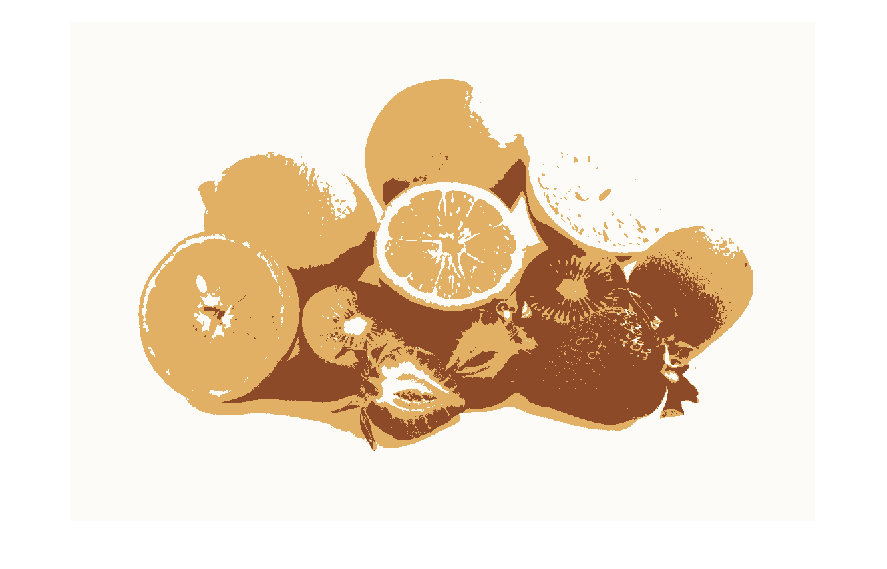
\includegraphics[width=\textwidth]{figures/k3_01.png}
      \caption{initial centroid: \\
      $
    \begin{bmatrix}
        255 & 255 & 255\\
        255 & 255 & 255\\
        233 & 213 & 150
    \end{bmatrix}
     $}  
\end{subfigure}
  \begin{subfigure}[b]{0.4\textwidth}
    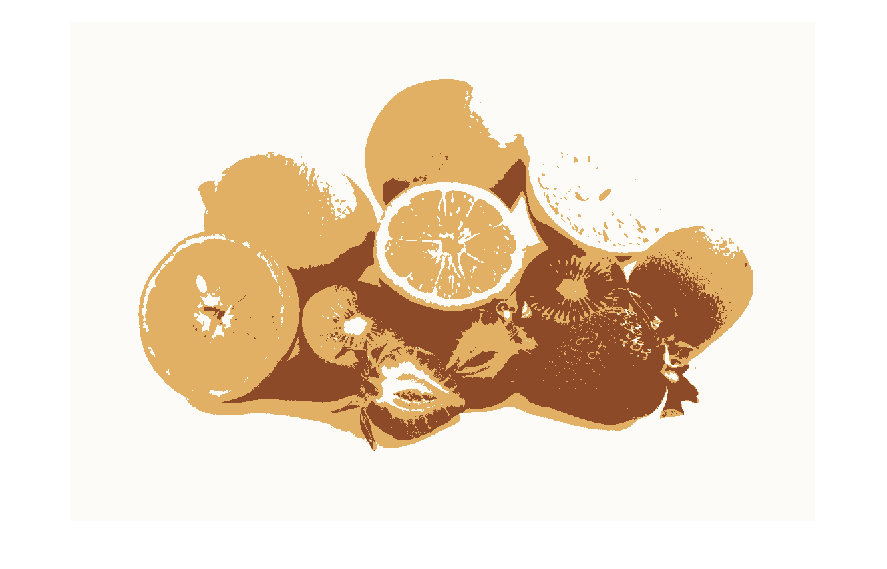
\includegraphics[width=\textwidth]{figures/k3_02.png}
      \caption{initial centroid: \\
      $
    \begin{bmatrix}
        255 & 152 & 29\\
        255 & 255 & 255\\
        255 & 255 & 255
    \end{bmatrix}
     $}
  \end{subfigure}
    \begin{subfigure}[b]{0.4\textwidth}
    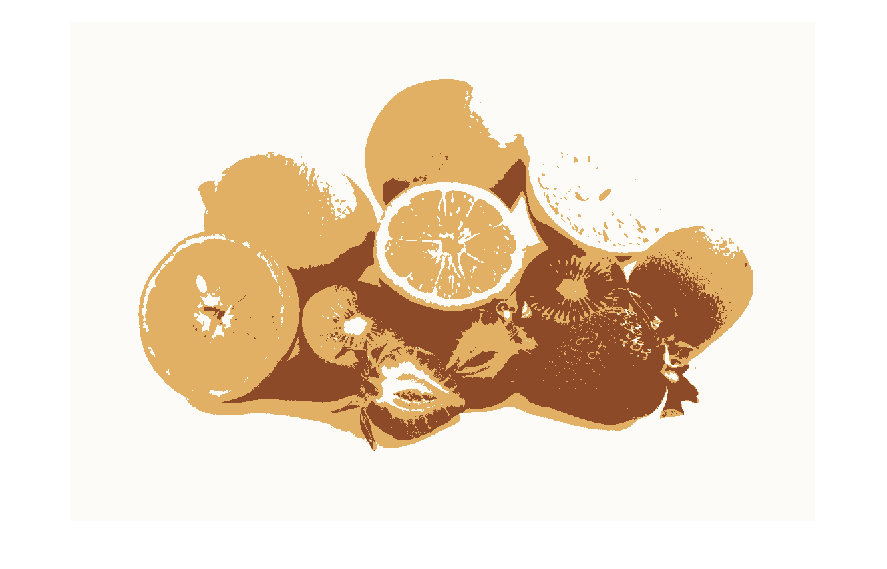
\includegraphics[width=\textwidth]{figures/k3_03.png}
      \caption{initial centroid: \\ 
      $
    \begin{bmatrix}
        255 & 255 & 255\\
        250 & 250 & 252\\
        255 & 255 & 255
    \end{bmatrix}
     $}
       \end{subfigure}
  \begin{subfigure}[b]{0.4\textwidth}
    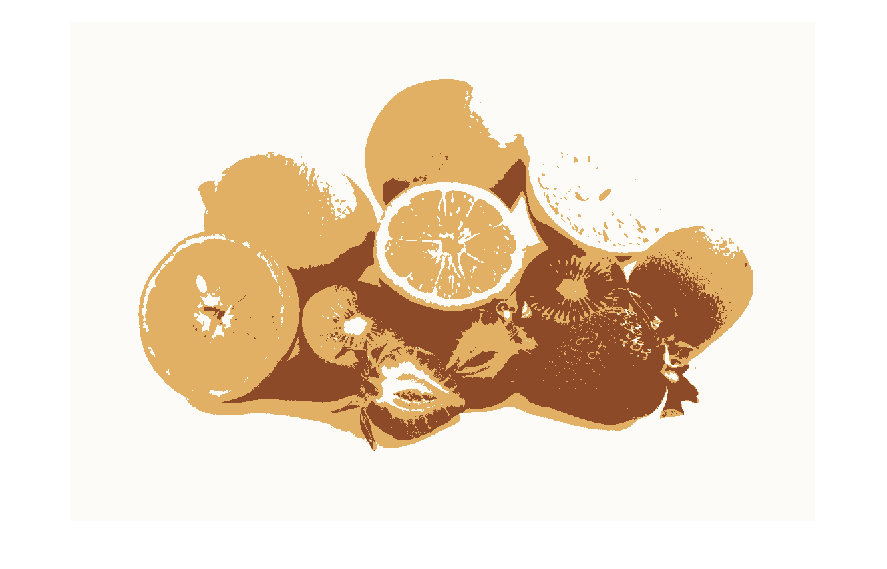
\includegraphics[width=\textwidth]{figures/k3_04.png}
      \caption{initial centroid: \\$
    \begin{bmatrix}
        255 & 255 & 255\\
        255 & 255 & 255\\
        255 & 255 & 255
    \end{bmatrix}
     $}
  \end{subfigure}
    \begin{subfigure}[b]{0.4\textwidth}
    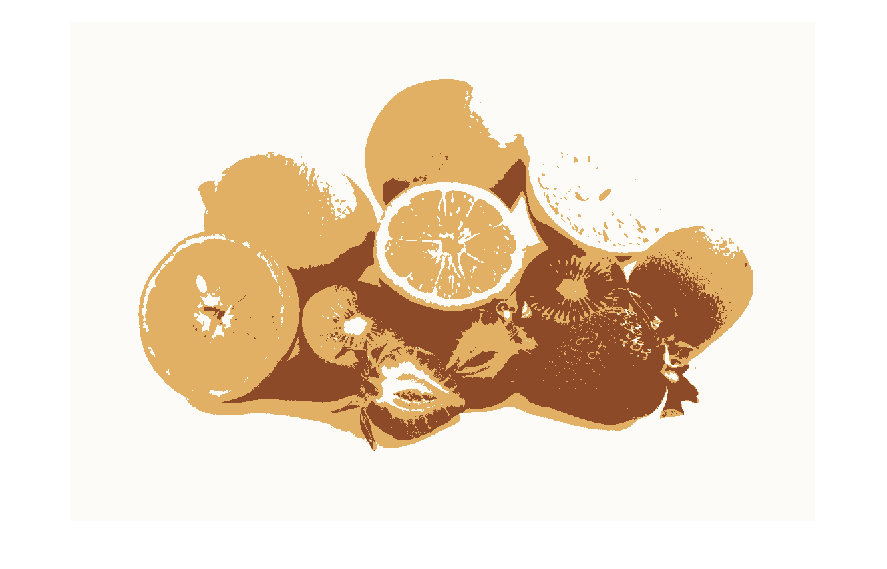
\includegraphics[width=\textwidth]{figures/k3_05.png}
      \caption{initial centroid: \\$
    \begin{bmatrix}
        143 & 5 & 21\\
        118 & 132 & 73\\
        228 & 156 & 48
    \end{bmatrix}
     $}
  \end{subfigure}
  \caption{Images with different distributed ray tracing effects}
  \label{kmeans}
\end{figure}


%%%%%%%%%%%%%% PROBLEM 2 %%%%%%%%%%%%%%%%%%%
\section{Object Recognition}
\subsection*{a,b}
The accuracy is around 72\%. Please refer to the code for implementation.

%%%%%%%%%%%%%%%%%%%%%%%%%%%%%%%%%%%%%%%%%%%%
%%%%%%%%%%%%%%%%%%%%%%%%%%%%%%%%%%%%%%%%%%%%
%%%%%%%%%%%%%%%%%%%%%%%%%%%%%%%%%%%%%%%%%%%%
%%%%%%%%%%%%%%%%%%%%%%%%%%%%%%%%%%%%%%%%%%%%
%%%%%%%%%%%%%%%%%%%%%%%%%%%%%%%%%%%%%%%%%%%%
%%%%%%%%%%%%%%%%%%%%%%%%%%%%%%%%%%%%%%%%%%%%

\end{document}
